% ============================================================================
%  BTP Presentation — SRAM-Fused Triton Kernel for MC Inventory Optimisation
%  IIT Kharagpur  |  Beamer (academic minimalist)
% ============================================================================
\documentclass[aspectratio=169, 11pt]{beamer}

% --- Theme: minimalist academic ---------------------------------------------
\usetheme{Madrid}
\usecolortheme{whale}
\usefonttheme{professionalfonts}

% Customise colours
\definecolor{iitkgp}{RGB}{0, 51, 102}
\definecolor{accent}{RGB}{192, 57, 43}
\definecolor{cpucol}{RGB}{120,144,168}
\definecolor{ptcol}{RGB}{232,168,56}
\definecolor{trcol}{RGB}{192,57,43}
\definecolor{inputmem}{RGB}{100,180,220}
\definecolor{dmem}{RGB}{70,130,180}
\definecolor{outmem}{RGB}{180,220,140}
\definecolor{goodgreen}{RGB}{46,125,50}

\setbeamercolor{structure}{fg=iitkgp}
\setbeamercolor{frametitle}{bg=iitkgp, fg=white}
\setbeamercolor{title}{bg=iitkgp, fg=white}
\setbeamercolor{block title}{bg=iitkgp!80, fg=white}
\setbeamercolor{block body}{bg=iitkgp!5}
\setbeamercolor{alerted text}{fg=accent}
\setbeamercolor{item}{fg=iitkgp}

\setbeamertemplate{navigation symbols}{}
\setbeamertemplate{footline}[frame number]
\setbeamertemplate{itemize items}[circle]
\setbeamertemplate{enumerate items}[default]

% --- Packages ---------------------------------------------------------------
\usepackage[utf8]{inputenc}
\usepackage[T1]{fontenc}
\usepackage{lmodern}
\usepackage{amsmath, amssymb, bm}
\usepackage{graphicx}
\graphicspath{{report_figures/}{diagrams/}}
\usepackage{booktabs}
\usepackage{tikz}
\usepackage{pgfplots}
\pgfplotsset{compat=1.18}
\usetikzlibrary{positioning, arrows.meta, calc, patterns, fit, shapes.geometric, decorations.pathreplacing}
\usepackage{appendixnumberbeamer}

\newcommand{\E}{\mathbb{E}}
\newcommand{\blockm}{\texttt{BLOCK\_M}}
\newcommand{\blockn}{\texttt{BLOCK\_N}}
\newcommand{\blockk}{\texttt{BLOCK\_K}}
\newcommand{\highlight}[1]{\textcolor{accent}{\textbf{#1}}}

\tikzset{
    stage blue/.style={rectangle, rounded corners=3pt, draw=blue!70!black, fill=blue!10, minimum width=2.6cm, minimum height=1.2cm, align=center, font=\small},
    stage green/.style={rectangle, rounded corners=3pt, draw=green!70!black, fill=green!10, minimum width=2.6cm, minimum height=1.2cm, align=center, font=\small},
    stage orange/.style={rectangle, rounded corners=3pt, draw=orange!70!black, fill=orange!10, minimum width=2.6cm, minimum height=1.2cm, align=center, font=\small},
    stage red/.style={rectangle, rounded corners=3pt, draw=red!70!black, fill=red!10, minimum width=2.6cm, minimum height=1.2cm, align=center, font=\small},
    step blue/.style={rectangle, rounded corners=3pt, draw=blue!70!black, fill=blue!10, minimum width=2.1cm, minimum height=0.7cm, align=center, font=\small},
    step green/.style={rectangle, rounded corners=3pt, draw=green!70!black, fill=green!10, minimum width=2.1cm, minimum height=0.7cm, align=center, font=\small},
    step orange/.style={rectangle, rounded corners=3pt, draw=orange!70!black, fill=orange!10, minimum width=2.1cm, minimum height=0.7cm, align=center, font=\small},
    step red/.style={rectangle, rounded corners=3pt, draw=red!70!black, fill=red!10, minimum width=2.1cm, minimum height=0.7cm, align=center, font=\small},
    step darkgreen/.style={rectangle, rounded corners=3pt, draw=green!80!black, fill=green!20!black!10, minimum width=2.1cm, minimum height=0.7cm, align=center, font=\small},
}

% --- Metadata ---------------------------------------------------------------
\title[SRAM-Fused Triton Kernel]{SRAM-Fused Triton Kernel for Monte-Carlo\\Inventory Optimisation}
\subtitle{A Multi-Echelon Stochastic Newsvendor Approach}
\author{Abhijit Kumar}
\institute[IIT KGP]{Department of Industrial and Systems Engineering\\Indian Institute of Technology Kharagpur\\\smallskip\textit{Supervisor: Dr.\ Abhishek Sharma}}
\date{April 2026}

% ============================================================================
\begin{document}

\begin{frame}[plain]
\titlepage
\end{frame}

\begin{frame}{Outline}
\tableofcontents
\end{frame}

% ============================================================================
\section{Introduction}
% ============================================================================

\begin{frame}{The Newsvendor Problem at Scale}
\begin{columns}[T]
\begin{column}{0.55\textwidth}
\textbf{Problem:} Optimal order quantity $Q$ under uncertain demand $D$
\begin{itemize}
    \item Order too little $\to$ lost sales
    \item Order too much $\to$ excess inventory
    \item Classical solution: $Q^* = F^{-1}\!\left(\frac{p-c}{p-s}\right)$
\end{itemize}
\vspace{0.5em}
\textbf{Our setting:}
\begin{itemize}
    \item \highlight{2,048} product-location nodes
    \item \highlight{131,072} Monte-Carlo scenarios
    \item Spatially correlated demand (real M5 dataset)
    \item Heavy-machinery dealership (tractors + generators)
\end{itemize}
\end{column}
\begin{column}{0.42\textwidth}
\begin{block}{Computational Bottleneck}
Intermediate demand matrix:
\[
\mathbf{D} = \bm{\mu} + \mathbf{L}\mathbf{Z}
\]
\begin{center}
$[2048 \times 131072] \times 4\text{B}$\\[0.3em]
$= $ \highlight{1.0\,GB} in FP32\\[0.3em]
{\small Must round-trip through HBM\\in standard PyTorch}
\end{center}
\end{block}
\end{column}
\end{columns}
\end{frame}

% ---------------------------------------------------------------------------
\begin{frame}{Core Idea: Kernel Fusion}
\begin{center}
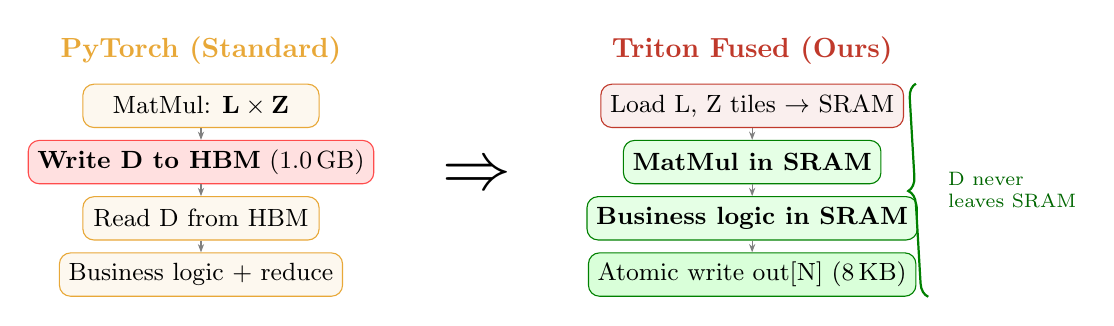
\begin{tikzpicture}[font=\small, node distance=0.4cm]
% PyTorch
\node[font=\normalsize\bfseries, text=ptcol] at (-3.5, 2.8) {PyTorch (Standard)};
\node[draw=ptcol, fill=ptcol!8, rounded corners, minimum width=3cm, minimum height=0.55cm] (a1) at (-3.5, 2.1) {MatMul: $\mathbf{L} \times \mathbf{Z}$};
\node[draw=red!70, fill=red!12, rounded corners, minimum width=3cm, minimum height=0.55cm, below=0.15cm of a1] (a2) {\textbf{Write D to HBM} (1.0\,GB)};
\node[draw=ptcol, fill=ptcol!8, rounded corners, minimum width=3cm, minimum height=0.55cm, below=0.15cm of a2] (a3) {Read D from HBM};
\node[draw=ptcol, fill=ptcol!8, rounded corners, minimum width=3cm, minimum height=0.55cm, below=0.15cm of a3] (a4) {Business logic + reduce};
\draw[-{Stealth[length=3pt]}, gray] (a1)--(a2);
\draw[-{Stealth[length=3pt]}, gray] (a2)--(a3);
\draw[-{Stealth[length=3pt]}, gray] (a3)--(a4);

% Arrow
\node[font=\Huge] at (0, 1.2) {$\Rightarrow$};

% Triton
\node[font=\normalsize\bfseries, text=trcol] at (3.5, 2.8) {Triton Fused (Ours)};
\node[draw=trcol, fill=trcol!8, rounded corners, minimum width=3.2cm, minimum height=0.55cm] (b1) at (3.5, 2.1) {Load L, Z tiles $\to$ SRAM};
\node[draw=green!50!black, fill=green!10, rounded corners, minimum width=3.2cm, minimum height=0.55cm, below=0.15cm of b1] (b2) {\textbf{MatMul in SRAM}};
\node[draw=green!50!black, fill=green!10, rounded corners, minimum width=3.2cm, minimum height=0.55cm, below=0.15cm of b2] (b3) {\textbf{Business logic in SRAM}};
\node[draw=green!50!black, fill=green!15, rounded corners, minimum width=3.2cm, minimum height=0.55cm, below=0.15cm of b3] (b4) {Atomic write out[N] (8\,KB)};
\draw[-{Stealth[length=3pt]}, gray] (b1)--(b2);
\draw[-{Stealth[length=3pt]}, gray] (b2)--(b3);
\draw[-{Stealth[length=3pt]}, gray] (b3)--(b4);

\draw[decorate, decoration={brace, amplitude=5pt, mirror}, thick, green!50!black] ([xshift=0.15cm]b1.north east) -- ([xshift=0.15cm]b4.south east) node[midway, right=0.2cm, font=\scriptsize, text=green!40!black, align=left] {D never\\leaves SRAM};
\end{tikzpicture}
\end{center}
\vspace{-0.5em}
{\centering\small \highlight{Key insight:} D is transient --- computed, consumed once, discarded. Inspired by FlashAttention.\par}
\end{frame}

% ============================================================================
\section{Methodology}
% ============================================================================

\begin{frame}{Data Pipeline}
\begin{center}
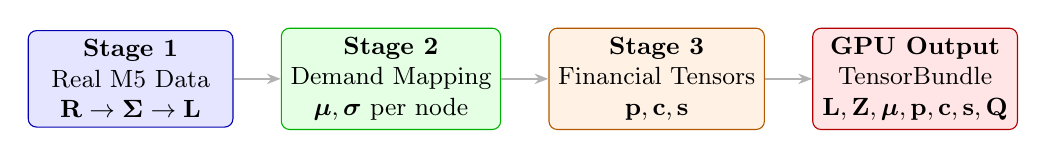
\begin{tikzpicture}[node distance=0.3cm and 0.5cm]
\node[stage blue] (s1) {\textbf{Stage 1}\\Real M5 Data\\$\mathbf{R} \to \bm{\Sigma} \to \mathbf{L}$};
\node[stage green, right=0.6cm of s1] (s2) {\textbf{Stage 2}\\Demand Mapping\\$\bm{\mu}, \bm{\sigma}$ per node};
\node[stage orange, right=0.6cm of s2] (s3) {\textbf{Stage 3}\\Financial Tensors\\$\mathbf{p}, \mathbf{c}, \mathbf{s}$};
\node[stage red, right=0.6cm of s3] (s4) {\textbf{GPU Output}\\TensorBundle\\$\mathbf{L}, \mathbf{Z}, \bm{\mu}, \mathbf{p}, \mathbf{c}, \mathbf{s}, \mathbf{Q}$};
\draw[-{Stealth[length=5pt]}, thick, draw=gray!60] (s1) -- (s2);
\draw[-{Stealth[length=5pt]}, thick, draw=gray!60] (s2) -- (s3);
\draw[-{Stealth[length=5pt]}, thick, draw=gray!60] (s3) -- (s4);
\end{tikzpicture}
\end{center}

\vspace{0.5em}
\begin{columns}[T]
\begin{column}{0.48\textwidth}
\begin{block}{Correlation Structure}
\small
Empirical Pearson correlation from \textbf{real M5 Kaggle dataset} --- 30K+ store-product daily sales series, trailing 365 days. Auto-downloaded via \texttt{kagglehub}.
\end{block}
\end{column}
\begin{column}{0.48\textwidth}
\begin{block}{Problem Scale}
\small
\begin{tabular}{ll}
Nodes ($N$) & 2,048 (60\% tractors, 40\% gen.) \\
Scenarios ($S$) & 131,072 ($2^{17}$) \\
$\mathbf{L}$ matrix & 16\,MB \\
$\mathbf{Z}$ matrix & 1.0\,GB \\
Precision & FP32 \\
\end{tabular}
\end{block}
\end{column}
\end{columns}
\end{frame}

% ---------------------------------------------------------------------------
\begin{frame}{Mathematical Framework}
\begin{block}{Expected Profit (Monte-Carlo SAA)}
\[
\E[\pi_i] = \frac{1}{S} \sum_{s=1}^{S} \Big[ p_i \cdot \underbrace{\min(D_{i,s}, Q_i)}_{\text{sales}} - c_i \cdot Q_i + s_i \cdot \underbrace{\max(Q_i - D_{i,s}, 0)}_{\text{overage}} \Big]
\]
where $D_{i,s} = \max\!\big(\mu_i + \sum_k L_{ik} Z_{ks},\; 0\big)$
\end{block}

\vspace{0.3em}
\begin{center}
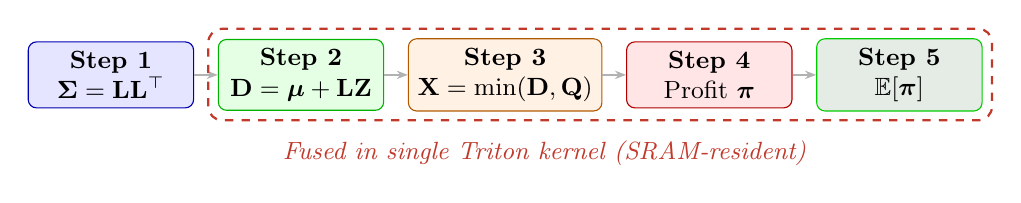
\begin{tikzpicture}[node distance=0.15cm and 0.3cm]
\node[step blue] (c1) {\textbf{Step 1}\\$\bm{\Sigma}=\mathbf{L}\mathbf{L}^\top$};
\node[step green, right=0.3cm of c1] (c2) {\textbf{Step 2}\\$\mathbf{D}=\bm{\mu}+\mathbf{L}\mathbf{Z}$};
\node[step orange, right=0.3cm of c2] (c3) {\textbf{Step 3}\\$\mathbf{X}=\min(\mathbf{D},\mathbf{Q})$};
\node[step red, right=0.3cm of c3] (c4) {\textbf{Step 4}\\Profit $\bm{\pi}$};
\node[step darkgreen, right=0.3cm of c4] (c5) {\textbf{Step 5}\\$\E[\bm{\pi}]$};
\draw[-{Stealth[length=4pt]}, thick, gray!60](c1)--(c2);
\draw[-{Stealth[length=4pt]}, thick, gray!60](c2)--(c3);
\draw[-{Stealth[length=4pt]}, thick, gray!60](c3)--(c4);
\draw[-{Stealth[length=4pt]}, thick, gray!60](c4)--(c5);
\draw[dashed, thick, accent, rounded corners=5pt] ([shift={(-0.12,-0.12)}]c2.south west) rectangle ([shift={(0.12,0.12)}]c5.north east);
\node[font=\small\itshape, accent, below=0.25cm of c3, xshift=0.5cm] {Fused in single Triton kernel (SRAM-resident)};
\end{tikzpicture}
\end{center}
\end{frame}

% ============================================================================
\section{Triton Kernel Design}
% ============================================================================

\begin{frame}{Kernel Architecture: 4-Phase Fusion}
\begin{center}
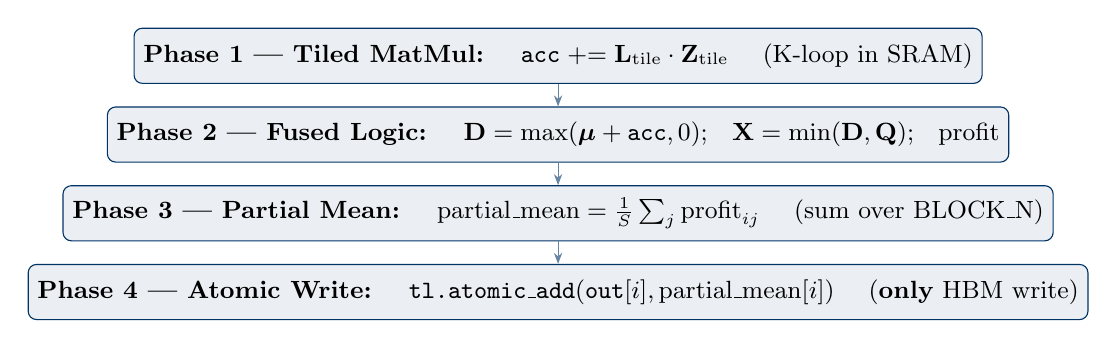
\begin{tikzpicture}[font=\small,
    phase/.style={rectangle, rounded corners=3pt, draw=iitkgp, fill=iitkgp!8, minimum width=10cm, minimum height=0.7cm, align=left},
]
\node[phase] (p1) at (0, 3.0) {\textbf{Phase 1 --- Tiled MatMul:} \quad $\texttt{acc} \mathrel{+}= \mathbf{L}_\text{tile} \cdot \mathbf{Z}_\text{tile}$ \quad (K-loop in SRAM)};
\node[phase] (p2) at (0, 2.0) {\textbf{Phase 2 --- Fused Logic:} \quad $\mathbf{D} = \max(\bm{\mu}+\texttt{acc}, 0)$; \; $\mathbf{X}=\min(\mathbf{D},\mathbf{Q})$; \; profit};
\node[phase] (p3) at (0, 1.0) {\textbf{Phase 3 --- Partial Mean:} \quad $\text{partial\_mean} = \frac{1}{S}\sum_j \text{profit}_{ij}$ \quad (sum over BLOCK\_N)};
\node[phase] (p4) at (0, 0.0) {\textbf{Phase 4 --- Atomic Write:} \quad $\texttt{tl.atomic\_add}(\texttt{out}[i], \text{partial\_mean}[i])$ \quad (\textbf{only} HBM write)};
\draw[-{Stealth[length=4pt]}, iitkgp!60] (p1)--(p2);
\draw[-{Stealth[length=4pt]}, iitkgp!60] (p2)--(p3);
\draw[-{Stealth[length=4pt]}, iitkgp!60] (p3)--(p4);
\end{tikzpicture}
\end{center}

\vspace{0.3em}
\begin{columns}[T]
\begin{column}{0.48\textwidth}
\begin{block}{Grid Decomposition}
\[
\text{Grid} = \left\lceil \frac{N}{\blockm}\right\rceil \times \left\lceil \frac{S}{\blockn}\right\rceil
\]
Each tile: $[\blockm, \blockn]$ of \textit{virtual} profit
\end{block}
\end{column}
\begin{column}{0.48\textwidth}
\begin{block}{SRAM Budget (T4: 48\,KB)}
\small
\begin{tabular}{lc}
L tile (BM$\times$BK$\times$4B) & 8\,KB \\
Z tile (BK$\times$BN$\times$4B) & 16\,KB \\
Accumulator (BM$\times$BN$\times$4B) & 32\,KB \\
\midrule
\textbf{Total} & \textbf{36\,KB} $\checkmark$ \\
\end{tabular}
\end{block}
\end{column}
\end{columns}
\end{frame}

% ============================================================================
\section{Results --- Kernel Performance}
% ============================================================================

\begin{frame}{Headline Results (N=2048, S=131072, Tesla T4)}
\begin{columns}[T]
\begin{column}{0.3\textwidth}
\begin{block}{\centering Memory Saved}
\begin{center}
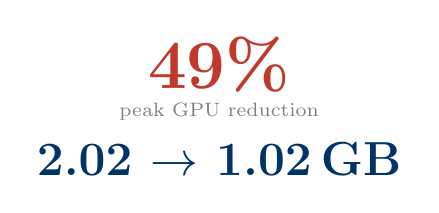
\begin{tikzpicture}
\node[font=\fontsize{32}{36}\selectfont\bfseries, text=accent] at (0,0.4) {49\%};
\node[font=\scriptsize, text=gray] at (0,-0.2) {peak GPU reduction};
\node[font=\fontsize{16}{20}\selectfont\bfseries, text=iitkgp] at (0,-0.8) {2.02 $\to$ 1.02\,GB};
\end{tikzpicture}
\end{center}
\end{block}
\end{column}
\begin{column}{0.3\textwidth}
\begin{block}{\centering HBM Traffic}
\begin{center}
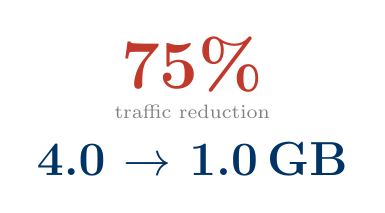
\begin{tikzpicture}
\node[font=\fontsize{32}{36}\selectfont\bfseries, text=accent] at (0,0.4) {75\%};
\node[font=\scriptsize, text=gray] at (0,-0.2) {traffic reduction};
\node[font=\fontsize{16}{20}\selectfont\bfseries, text=iitkgp] at (0,-0.8) {4.0 $\to$ 1.0\,GB};
\end{tikzpicture}
\end{center}
\end{block}
\end{column}
\begin{column}{0.3\textwidth}
\begin{block}{\centering vs CPU}
\begin{center}
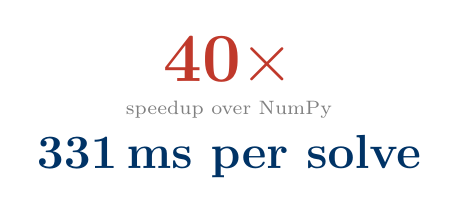
\begin{tikzpicture}
\node[font=\fontsize{32}{36}\selectfont\bfseries, text=accent] at (0,0.4) {40$\times$};
\node[font=\scriptsize, text=gray] at (0,-0.2) {speedup over NumPy};
\node[font=\fontsize{16}{20}\selectfont\bfseries, text=iitkgp] at (0,-0.8) {331\,ms per solve};
\end{tikzpicture}
\end{center}
\end{block}
\end{column}
\end{columns}

\vspace{0.3em}
\begin{center}
\footnotesize
\begin{tabular}{lccc}
\toprule
& \textbf{CPU-NumPy} & \textbf{PyTorch-Compile} & \textbf{Triton-Fused (Ours)} \\
\midrule
Time (ms) & 13{,}233 & 258 & 331 \\
Peak GPU Mem & N/A & 2.024\,GB & \highlight{1.024\,GB} \\
\bottomrule
\end{tabular}
\end{center}
\end{frame}

% ---------------------------------------------------------------------------
\begin{frame}{Memory Efficiency --- Primary Contribution}
\begin{columns}[T]
\begin{column}{0.5\textwidth}
\begin{center}
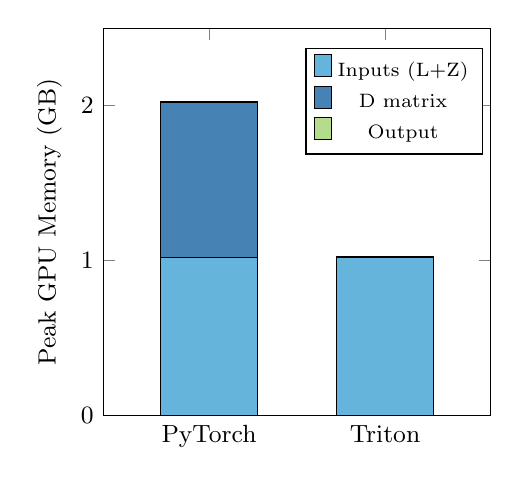
\begin{tikzpicture}
\begin{axis}[
    ybar stacked, bar width=35pt, width=6.5cm, height=6.5cm,
    ylabel={Peak GPU Memory (GB)}, ylabel style={font=\small},
    symbolic x coords={PyTorch, Triton},
    xtick=data, xticklabel style={font=\small},
    ymin=0, ymax=2.5,
    tick label style={font=\small},
    legend style={font=\scriptsize, at={(0.98,0.95)}, anchor=north east},
    enlarge x limits=0.6,
]
\addplot[fill=inputmem] coordinates {(PyTorch,1.02) (Triton,1.02)};
\addplot[fill=dmem]     coordinates {(PyTorch,1.00) (Triton,0.0)};
\addplot[fill=outmem]   coordinates {(PyTorch,0.004) (Triton,0.004)};
\legend{Inputs (L+Z), D matrix, Output}
\end{axis}
\end{tikzpicture}
\end{center}
\end{column}
\begin{column}{0.46\textwidth}
\vspace{0.3cm}
\begin{block}{Key Takeaway}
\small
D matrix = \highlight{1.0\,GB} in PyTorch, \textbf{completely eliminated} by Triton $\to$ \highlight{49.4\%} peak memory reduction.
\end{block}
\vspace{0.3em}
\begin{block}{Why It Matters}
\small
At $N{=}10{,}000$: D would be 40\,GB --- fused approach becomes the \textbf{only} viable single-GPU solution.
\end{block}
\end{column}
\end{columns}
\end{frame}

% ---------------------------------------------------------------------------
\begin{frame}{Scaling Behaviour ($S{=}65{,}536$ fixed)}
\begin{columns}[T]
\begin{column}{0.52\textwidth}
\vspace{-0.3cm}
\begin{center}

\includegraphics[width=\textwidth]{scaling_sweep.png}
\end{center}
\end{column}
\begin{column}{0.45\textwidth}
\footnotesize
\begin{tabular}{rrr}
\toprule
$N$ & \textbf{Speedup} & \textbf{Mem Savings} \\
\midrule
128  & 1.1$\times$ & 2.9\%  \\
256  & 1.1$\times$ & 5.4\%  \\
512  & 1.5$\times$ & 9.8\%  \\
1024 & 1.0$\times$ & 16.4\% \\
2048 & 0.8$\times$ & 24.5\% \\
\bottomrule
\end{tabular}

\vspace{0.4em}
\begin{block}{Key Finding}
\footnotesize
\textbf{Memory savings grow with $N$} as $\mathbf{D}[N,S]$ becomes a larger fraction of total memory. Speedup peaks at moderate $N$; at large $N$ the matmul dominates. Extension kernels achieve clear speedups at all scales.
\end{block}
\end{column}
\end{columns}
\end{frame}

% ---------------------------------------------------------------------------
\begin{frame}{Numerical Correctness}
\begin{center}
\begin{tabular}{lccc}
\toprule
\textbf{Comparison} & \textbf{Max Abs Diff} & \textbf{Mean Abs Diff} & \textbf{Status} \\
\midrule
CPU vs PyTorch    & 0.002441 & 0.000125 & \textcolor{goodgreen}{\textbf{PASS}} \\
CPU vs Triton     & 0.004883 & 0.000215 & \textcolor{goodgreen}{\textbf{PASS}} \\
PyTorch vs Triton & 0.004883 & 0.000234 & \textcolor{goodgreen}{\textbf{PASS}} \\
\bottomrule
\end{tabular}
\end{center}

\vspace{0.8em}
\begin{block}{Validation Protocol}
\begin{itemize}
    \item \texttt{torch.allclose} with $\texttt{atol}=10^{-2}$, $\texttt{rtol}=10^{-3}$
    \item All three solvers agree within FP32 tolerance
    \item Small discrepancies from non-deterministic atomic reduction order
\end{itemize}
\end{block}
\end{frame}

% ============================================================================
\section{Results --- Extension Kernels}
% ============================================================================

\begin{frame}{Extension Kernels: Performance \& Memory}
\begin{center}
\small
\begin{tabular}{lrrrrr}
\toprule
\textbf{Extension} & \textbf{PT (ms)} & \textbf{TR (ms)} & \textbf{Speedup} & \textbf{TR Mem} & \textbf{Mem $\downarrow$} \\
\midrule
Grid Search ($K{=}64$)   & 562 & 417 & \textcolor{goodgreen}{\textbf{1.3$\times$}} & 1.03\,GB & \textcolor{goodgreen}{\textbf{66\%}} \\
CVaR ($\alpha{=}0.05$)   & 634 & 384 & \textcolor{goodgreen}{\textbf{1.7$\times$}} & 1.03\,GB & \textcolor{goodgreen}{\textbf{90\%}} \\
Budget (bisection)       & ---   & 18{,}123 & ---         & 1.03\,GB & --- \\
Substitution (2-pass)    & 305 & 756 & 0.4$\times$ & 2.03\,GB & 0\% \\
\bottomrule
\end{tabular}
\end{center}

\vspace{0.5em}
\begin{block}{Architecture Insight}
\begin{itemize}
    \item \textbf{Single-pass kernels} (Grid Search, CVaR) achieve 1.3--1.7$\times$ speedup because more work is fused per matmul tile (K Q-values, histogram binning)
    \item \textbf{CVaR: 90\% memory reduction} --- PyTorch needs ${\sim}$10\,GB for profit matrix + quantile sort; Triton computes histogram in-SRAM
    \item \textbf{Two-pass Substitution} writes stockout$[N,S]$ to HBM between passes --- an honest finding about the \textit{limits} of SRAM fusion
\end{itemize}
\end{block}
\end{frame}

% ============================================================================
\section{Results --- Optimisation Quality}
% ============================================================================

\begin{frame}{Grid Search: Optimal $Q^*$ ($K{=}64$)}
\begin{columns}[T]
\begin{column}{0.48\textwidth}
\vspace{-0.4cm}
\begin{center}
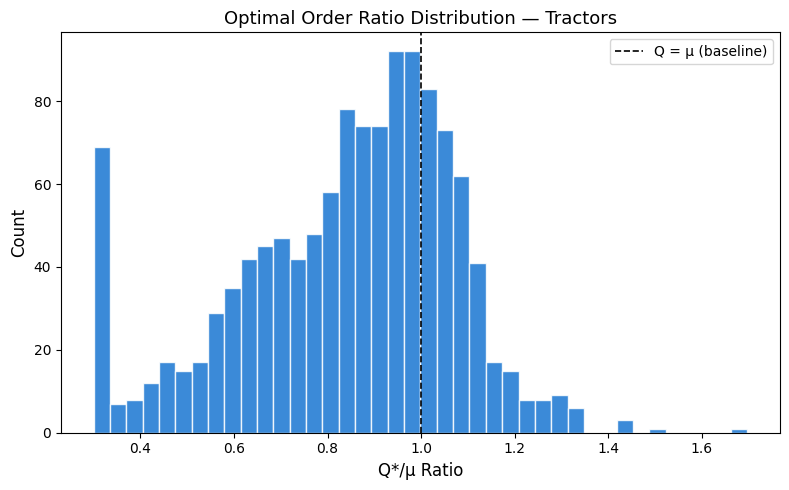
\includegraphics[width=0.88\textwidth]{gs_qstar_ratio_tractors.png}
\end{center}
\end{column}
\begin{column}{0.48\textwidth}
\vspace{-0.4cm}
\begin{center}
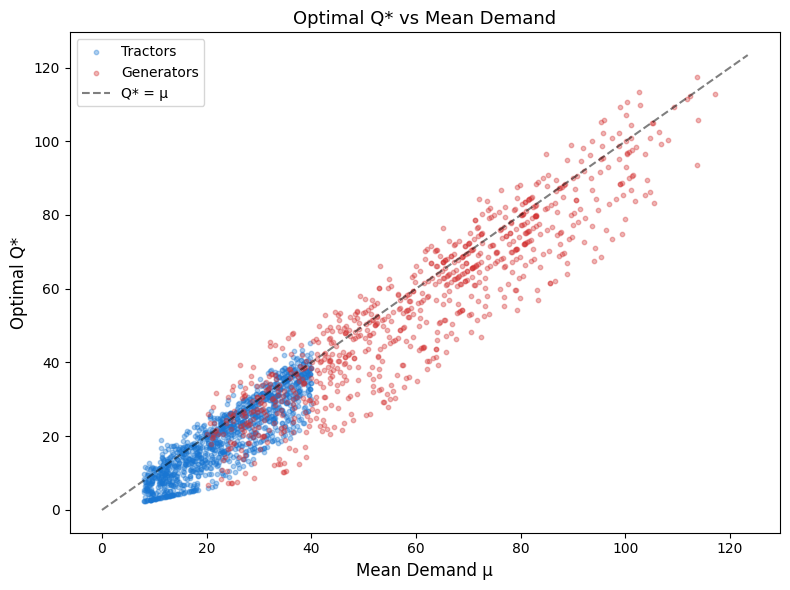
\includegraphics[width=0.88\textwidth]{gs_qstar_vs_mu_scatter.png}
\end{center}
\end{column}
\end{columns}

\vspace{-0.4em}
{\small\textbf{Key:} 78\% of products should order below $\mu$ (mean $Q^*/\mu = 0.854$). Aggregate profit: \highlight{+5.3\%}. Tractors $Q^*/\mu{=}0.825$; Generators $0.899$.}
\end{frame}

% ---------------------------------------------------------------------------
\begin{frame}{CVaR Risk Analysis ($\alpha{=}0.05$)}
\begin{columns}[T]
\begin{column}{0.48\textwidth}
\vspace{-0.3cm}
\begin{center}
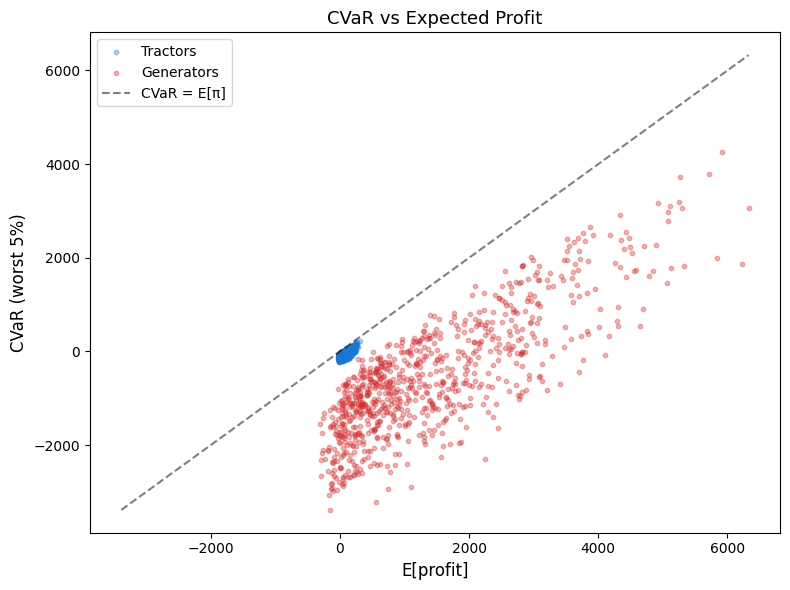
\includegraphics[width=0.95\textwidth]{cvar_vs_eprofit_scatter.png}
\end{center}
\end{column}
\begin{column}{0.48\textwidth}
\vspace{-0.3cm}
\begin{center}
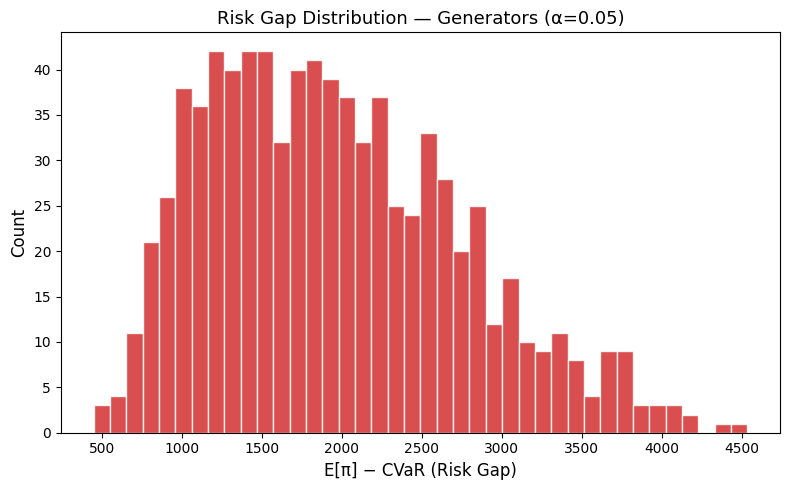
\includegraphics[width=0.95\textwidth]{cvar_risk_gap_generators.png}
\end{center}
\end{column}
\end{columns}

\vspace{-0.2em}
\begin{block}{Key Findings}
\small
\begin{itemize}\setlength\itemsep{0.1em}
    \item Generators carry \highlight{17.5$\times$ more tail risk} (mean gap 1{,}955 vs 112)
    \item $\text{CVaR} \leq \E[\pi]$: \textcolor{goodgreen}{\textbf{PASS}} for all 2,048 products
\end{itemize}
\end{block}
\end{frame}

% ---------------------------------------------------------------------------
\begin{frame}{Budget Constraint \& Substitution}
\begin{columns}[T]
\begin{column}{0.48\textwidth}
\begin{center}
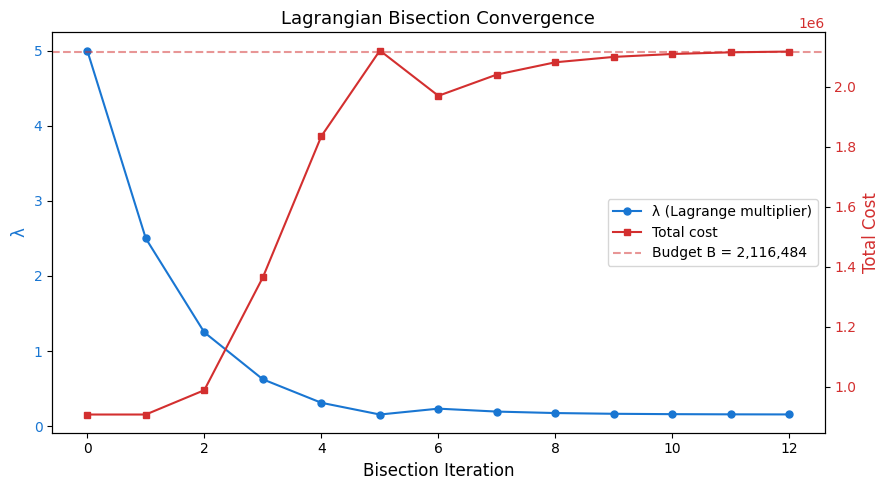
\includegraphics[width=\textwidth]{budget_bisection_convergence.png}
\end{center}
\vspace{-0.3em}
{\small\textbf{Budget:} Bisection converges in \textbf{13 iterations}.\\ $\lambda^*{=}0.1575$, aggregate profit loss $-30.7\%$.\\ Tractors absorb more constraint.}
\end{column}
\begin{column}{0.48\textwidth}
\begin{center}
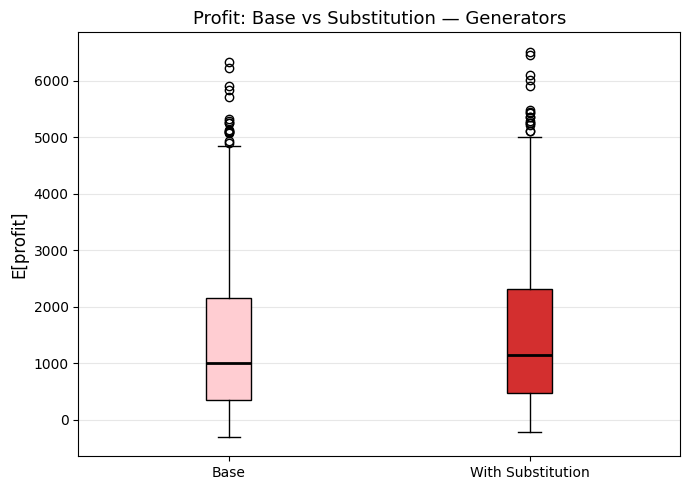
\includegraphics[width=\textwidth]{sub_boxplot_generators.png}
\end{center}
\vspace{-0.3em}
{\small\textbf{Substitution:} \highlight{+10.3\%} aggregate profit.\\ All 2,048 products benefit.\\ Generators redirect 1.8$\times$ more demand.}
\end{column}
\end{columns}
\end{frame}

% ============================================================================
\section{Conclusions}
% ============================================================================

\begin{frame}{Summary of Contributions}
\begin{enumerate}
    \item \textbf{Memory-efficient kernel fusion for inventory optimisation}\\
    49.4\% peak memory reduction; D$[N,S]$ eliminated from HBM; $\sim$75\% traffic reduction
    \vspace{0.3em}
    \item \textbf{Extension kernel speedups}\\
    Grid Search 1.3$\times$ (66\% mem $\downarrow$), CVaR 1.7$\times$ (90\% mem $\downarrow$)
    \vspace{0.3em}
    \item \textbf{Real data pipeline}\\
    M5 Kaggle dataset correlations + heavy-machinery financial parameters
    \vspace{0.3em}
    \item \textbf{Actionable optimisation insights}\\
    +5.3\% profit from $Q^*$; 17.5$\times$ tail risk asymmetry; +10.3\% from substitution
    \vspace{0.3em}
    \item \textbf{Honest architectural analysis}\\
    Two-pass substitution kernel delineates the boundary of SRAM fusion
\end{enumerate}
\end{frame}

% ---------------------------------------------------------------------------
\begin{frame}{Future Work}
\begin{columns}[T]
\begin{column}{0.48\textwidth}
\begin{block}{Technical}
\begin{itemize}
    \item Differentiable simulation for end-to-end $Q$ optimisation
    \item Mixed-precision (FP16/BF16 on Ampere/Hopper)
    \item Multi-GPU scaling for $N > 10{,}000$
    \item Single-pass substitution kernel
\end{itemize}
\end{block}
\end{column}
\begin{column}{0.48\textwidth}
\begin{block}{Application}
\begin{itemize}
    \item Multi-period models with carry-over inventory
    \item Deployment study with real dealership network
    \item Real-time ERP integration (sub-second execution)
    \item Dynamic pricing extensions
\end{itemize}
\end{block}
\end{column}
\end{columns}

\vspace{0.8em}
\begin{center}
\large\textbf{Thank You}\\[0.3em]
\normalsize Questions?
\end{center}
\end{frame}

\end{document}
